\documentclass[../thesis.tex]{subfiles}
\begin{document}

\chapter{validation}
\label{chp:validation}

Within this chapter the model validation is explained and described. At first the experimental setup used in the performed experiments is shown and then the experimental and model results are explained. After that a comparison is done to show that the model is performing as expected.

\section{experimental setup}

The experiments used for validating the developed model where done using a sounding rocket as part of the \texttt{MORABA} (\textbf{Mo}bile \textbf{Ra}cketen \textbf{Ba}sis) \cite{stamminger2012moraba} setup. The mission's name was \texttt{TEXUS-57}. The experimental setup as shown in \cite{stergiou2022effects} is visible in \autoref{fig: experiment}.
\begin{figure}[htbp]
	\centering
	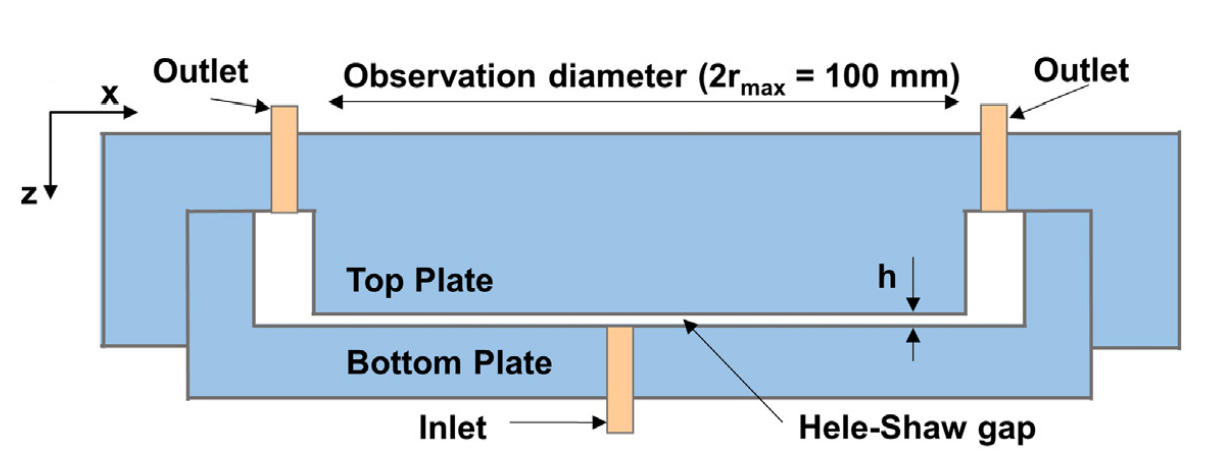
\includegraphics[scale=0.4]{experimental_setup}
	\caption{experimental setup for validation}
	\label{fig: experiment}
\end{figure}
The gap height $h$ used in the experiment for comparison with the model is 0.2 mm. 

\section{experimental results}

\section{model results}
\label{sec: model res}

\section{comparison}

\end{document}